Orijentacija osa koordinatnog sistema preko kojih su određeni 
vektori ili tenzori potpuno je proizvoljna. Obično se jedna od osi(e.g. $x$ osa) poravnava 
sa geometrijskom osom tijela. 
Ako se tijelo kreće stalnom brzinom tada se jedan koordinatni sistem može 
koristiti za sve veličine, međutim ako se tijelo rotira tada se naslućuju dva koordinatna sistema:
\begin{itemize}
    \item Koordinatni sistem vezan za zemlju
    \item Koordinatni sistem vezan za tijelo
\end{itemize}

Koordinatni sistem vezan za zemlju je inertcijalni iako se zemlje rotira u odnosu na geomtrijsku osu.
Sastoji se od tri ordinate, jedna predstavlja poziciju po sjevernoj osi, jedna po lokaloj istočnoj osi 
i jedna predstavlja vertikalnu poziciju. Ose koordinatnog sistema vezanog za zemlju su 
označene sa $X_e, Y_e, Z_e$. Drugim riječima, $X_e$ i $Y_e$ leže u ravni dok je $Z_e$ usmjeren ka centru Zemlje.\\
Koordinatni sistem vezan za tijelo sastoji se iz tri ordinate sa ishodištem u centru gravitacije letjelice: $x$ osa koja je
usmjerena ka nosu letjelice tj. podudara se sa longitudinalnom osom, $y$ ose koja je usmjerena ka desnom krilu letjelice i $z$ ose koja dopunjava lijevo orijentisani 
koordinatni sistem.
\begin{figure}[h!]
    \centering
    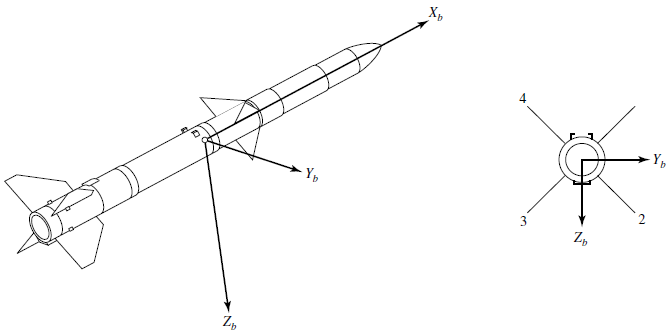
\includegraphics[scale=0.7]{body.png}
    \caption{Koordinatni sistem vezan za tijelo}
\end{figure}

Da se definiše položaj letjelice u odnosu na koordinatni sistem koriste se Eulerovi uglovi($\psi, \theta, \phi$).

\begin{figure}[h!]
    \centering
    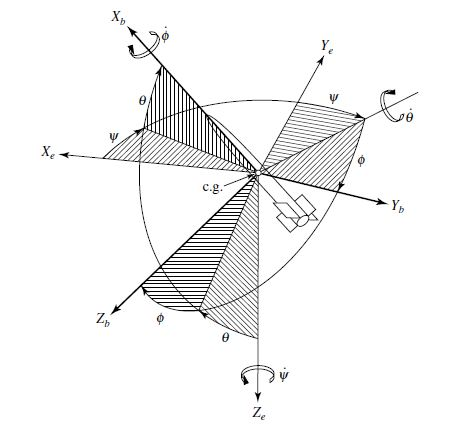
\includegraphics[scale=0.7]{earth-body.JPG}
    \caption{Eulerovi uglovi}
\end{figure}



